\documentclass[a4paper, 12pt]{article}

%Class
	%\documentclass[a4paper,12pt]{article}

%Packages
	\usepackage{amsmath}					% Standard maths
	\usepackage{amssymb}					% Standard maths
	\usepackage{amsthm}						% Standard maths
	\usepackage{thmtools, thm-restate}% Theorem styles
	\usepackage{mathtools}
	\usepackage[newzealand]{babel}% Date/time in British format (yes, I know it says NZ)
	\usepackage{datetime}					% Date/time
	\usepackage{multirow}					% For stacked subscripts
	\usepackage{xcolor}						% For colour!
	\usepackage[normalem]{ulem}		% For strikeout
	\usepackage{isomath}
	\usepackage{fancyhdr}					% For the headers
	\usepackage{mfirstuc}					% For the headers
	\usepackage[hmargin=1in,top=0.8in,bottom=1in]{geometry} % Page margins more reasonable
	\usepackage{graphicx}					% For including graphics
	%\usepackage{float}						% For something
	\usepackage{enumitem}					% For numbering tweaks
	\usepackage[margin=15pt,font={footnotesize},labelfont=bf,format=hang]{caption}
\usepackage[margin=15pt,font={footnotesize},labelfont=bf,format=hang]{subcaption}
	\usepackage{url}
	\usepackage[hidelinks]{hyperref}	% For hyperlinks
	\usepackage{breakurl}
	\usepackage{cleveref}
	\usepackage[scaled=.92]{helvet}
	\newbool{show_question}
	\newbool{show_solution}
	\newcommand{\solutioninheading}{\ifbool{show_solution}{: SOLUTIONS}{}}
	\usepackage{pgfplots}
\newcommand{\ep}{\varepsilon}

\makeatletter 
\newcommand\mynobreakpar{\par\nobreak\@afterheading} 
\makeatother

    \newcommand{\question}[3]{
    	\item \textbf{#1} \mynobreakpar \nobreak \medskip % Title
    	%
    	\ifbool{show_question}{\nobreak#2}{} % Question
    	%
    	%
    	\ifbool{show_question}{\ifbool{show_solution}{\par\medskip\textbf{Solution:}}{}}{} % Both
    	\ifbool{show_solution}{#3}{} % Answer
    }		

%MATHEMATICAL SHORTCUTS
%Two and three-part definitions
	\newcommand{\twopartdef}[4]
	{	\left\{
			\begin{array}{ll}
				#1 & \mbox{if } #2 \\
				#3 & \mbox{if } #4
			\end{array}
		\right.}
%	\newcommand{\threepartdef}[6]
%	{	\left\{
%			\begin{array}{ll}
%				#1 & \mbox{if } #2 \\
%				#3 & \mbox{if } #4 \\
%				#5 & \mbox{if } #6
%			\end{array}
%		\right.}
%Blackboard bold	
	\newcommand{\N}{{\mathbb N}} 
	\newcommand{\R}{{\mathbb R}} 
	\newcommand{\C}{{\mathbb C}} 
	%Curly letters
%	\newcommand{\E}{{\mathcal E}}	
%	\newcommand{\F}{{\mathcal F}} 
%	\newcommand{\Null}{{\mathcal N}} 
%	\newcommand{\R}{\mathcal{R}} 
%	\newcommand{\Z}{\mathcal{Z}} 
%Uprights
	\newcommand{\D}{{\mathrm D}}
	\renewcommand{\d}{{\mathrm d}}
%Easy Greeks
%	\def\a{\alpha}
%	\def\g{\gamma}
%	\newcommand{\e}{{\varepsilon}}
%	\newcommand{\la}{{\lambda}}  
%	\newcommand{\om}{{\Omega}}
	\renewcommand{\epsilon}{\varepsilon}
	
%Vector operators
	\def \p {\partial}
	\newcommand{\del}{{\nabla}}
	\newcommand{\grad}{{\nabla}}
    \newcommand{\vdel}{\boldsymbol{\nabla}}
    \newcommand{\vgrad}{\boldsymbol{\nabla}}
    \newcommand{\vnabla}{\boldsymbol{\nabla}}
	\newcommand{\cross}{{\times}}
	\newcommand{\Lap}{{\nabla^2}} 
%Arrows
%	\newcommand{\goesto}[1]{\xrightarrow[#1]{}}
%hats
%	\newcommand{\nhat}{\widehat{\v{n}}}
%	\newcommand{\shat}{\widehat{\v{s}}}
	\renewcommand{\hat}{\widehat}
%Note to self
%	\newcommand{\note}[1]{[\textbf{\textsl{\MakeUppercase{#1}}}]}
	
%Stress tensor
%	\newcommand{\T}{\vg{\sigma}}

% Vectors, quaternions etc.
\renewcommand{\v}[1]{\mathbfit{#1}}      % Generic vector
\newcommand{\vc}[1]{\bm{\mathcal{#1}}}      % vector mathcal
\newcommand{\uv}[1]{\widehat{\mathbfit{#1}}}      % Generic unit vector
\newcommand{\q}[1]{\mathsfbfit{#1}}        % Generic quaternion
\renewcommand{\t}[1]{\mathsfbfit{#1}}	 % Generic tensor
\newcommand{\m}[1]{\mathsfbfit{#1}}	 % Generic matrix
\newcommand{\vu}[1]{\mathbf{#1}}         % Upright vector (for zero vector)
\newcommand{\qu}[1]{\mathbf{#1}}       % Upright quaternion (for zero quaternion)
\newcommand{\tu}[1]{\bm{\mathsf{#1}}}	 % Upright tensor (for zero tensor)

%Real and imaginary
\renewcommand{\Re}{\operatorname{Re}}
\renewcommand{\Im}{\operatorname{Im}}
	
%Non-dim numbers
%	\renewcommand{\Re}{\operatorname{Re}}
%	\newcommand{\Bi}{\operatorname{Bi}}
%	\newcommand{\Fo}{\operatorname{Fo}}
	
%Misc
\DeclareMathSymbol{\Delta}{\mathalpha}{operators}{1} % Keeps Delta upright
\DeclareMathSymbol{\Gamma}{\mathalpha}{operators}{0} % Keeps Gamma upright
	\newcommand{\cosec}{\operatorname{cosec}}
	\newcommand{\cosech}{\operatorname{cosech}}
	\newcommand{\sech}{\operatorname{sech}}
	\newcommand{\tr}{\operatorname{tr}}
	\newcommand{\erf}{\operatorname{erf}}
	\newcommand{\order}{\mathcal{O}}
%	\newcommand{\V}{\mathcal{V}} % 	CurlyV = (Bi V) / (1 + Bi)

% Differentiating 
\newcommand{\fd}[2]{\mathchoice{\frac{\d #1}{\d #2}}{\d #1/\d #2}{\d #1/\d #2}{\d #1/\d #2}}
\newcommand{\fdd}[2]{\mathchoice{\frac{\d^2 #1}{\d #2^2}}{\d^2 #1/\d #2^2}{\d^2 #1/\d #2^2}{\d^2 #1/\d #2^2}}
\newcommand{\fddd}[2]{\mathchoice{\frac{\d^3 #1}{\d #2^3}}{\d^3 #1/\d #2^3}{\d^3 #1/\d #2^3}{\d^3 #1/\d #2^3}}
\newcommand{\fdddd}[2]{\mathchoice{\frac{\d^4 #1}{\d #2^4}}{\d^4 #1/\d #2^4}{\d^4 #1/\d #2^4}{\d^4 #1/\d #2^4}}
\newcommand{\fdn}[3]{\mathchoice{\frac{\d^{#1} #2}{\d #3^{#1}}}{\d^{#1} #2/\d #3^{#1}}{\d^{#1} #2/\d #3^{#1}}{\d^{#1} #2/\d #3^{#1}}}
\newcommand{\pd}[2]{\mathchoice{\frac{\p #1}{\p #2}}{\p #1/\p #2}{\p #1/\p #2}{\p #1/\p #2}}
\newcommand{\pdd}[2]{\mathchoice{\frac{\p^2 #1}{\p #2^2}}{\p^2 #1/\p #2^2}{\p^2 #1/\p #2^2}{\p^2 #1/\p #2^2}}
\newcommand{\pddmixed}[3]{\frac{\p^2 #1}{\p #2 \p #3}}
\newcommand{\pddd}[2]{\frac{\p^3 #1}{\p #2^3}}
\newcommand{\pdn}[3]{\mathchoice{\frac{\p^{#1} #2}{\p #3^{#1}}}{\p^{#1} #2/\p #3^{#1}}{\p^{#1} #2/\p #3^{#1}}{\p^{#1} #2/\p #3^{#1}}}
	
	% Misc
\newcommand{\e}{\mathrm{e}}
\renewcommand{\i}{\mathrm{i}}
\newcommand{\dx}{\,\mathrm{d}x}
\newcommand{\dy}{\,\mathrm{d}y}
\renewcommand{\epsilon}{\varepsilon}
\renewcommand{\Re}{\operatorname{Re}}
\newcommand{\Four}{\mathcal{F}}

\newcommand{\mat}[4]{\begin{pmatrix}#1 & #2 \\ #3 & #4 \end{pmatrix}}

	%Column vectors
	\makeatletter
\newcommand\rcvector[2][\\]{\ensuremath{%
  \global\def\rc@delim{#1}%
    \negthinspace\begin{pmatrix}
      \rc@vector #2,\relax\noexpand\@eolst%
    \end{pmatrix}}}
\def\rc@vector #1,#2\@eolst{%
  \ifx\relax#2\relax
    #1
  \else
    #1\rc@delim
    \rc@vector #2\@eolst%
  \fi}
\makeatother

\newcommand{\colvec}{\rcvector}
\newcommand{\rowvec}{\rcvector}
\renewcommand{\binom}{\rcvector}
	
	%Colours
%	\newcommand{\orange}[1]{{\color{orange} #1 }}
%	\newcommand{\blue}[1]{{\color{blue} #1 }}

%Theorem styles
%	\declaretheoremstyle[headpunct={\:\:\:}, shaded={bgcolor={rgb}{0.9,0.9,0.9}, margin=5pt}]{problem}
%	\declaretheoremstyle[headpunct={\:\:\:}, shaded={rulecolor=black, rulewidth=0.4pt, bgcolor={rgb}{1,1,1}, margin=5pt}]{definition}
%	\declaretheoremstyle[headpunct={\:\:\:}, spaceabove=15pt, notefont=\bf, notebraces={(}{)}]{theorem}
%	\declaretheoremstyle[headpunct={\:\:\:}, numbered=no, spaceabove=15pt, qed={\checkmark}]{solution}
%	
%	\declaretheorem[style=definition,numberwithin=section]{definition}
%	\declaretheorem[numberlike=definition, style=theorem]{theorem}
%	\declaretheorem[numberlike=definition, style=theorem]{lemma}
%	\declaretheorem[numberlike=definition,style=problem]{problem}
%	\declaretheorem[numberlike=definition, style=theorem]{proposition}
%	\declaretheorem[numberlike=definition, style=theorem]{corollary}
%	\declaretheorem[numberlike=definition, style=theorem]{remark}
%	\declaretheorem[numberlike=definition, style=theorem]{example}
%	\declaretheorem[numberlike=definition, style=theorem]{notation}
%	\declaretheorem[style=solution]{solution}

%Depth of display breaks to allow	
	\allowdisplaybreaks[1]

%How deep do we want the Table of Contents to go?	
%	\setcounter{tocdepth}{1}

%Sections
\makeatletter
\renewcommand{\section}{\@startsection
{section}%                   % the name
{1}%                         % the level
{0mm}%                       % the indent
{-\baselineskip}%            % the before skip
{0.5\baselineskip}%          % the after skip
{\normalfont\bfseries}} % the style
\makeatother

% Wavy underline
\makeatletter
\font\sixly=lasyb10 scaled 1200
\def\tinners{\bgroup \markoverwith{\lower8.5\p@\hbox{\sixly \char58}}\ULon}
\makeatother
\newcommand{\answer}[1]{\tinners{\; #1 \;}}

%Setting the footnotes to use *,**,+ etc rather than 1,2,3	
\renewcommand{\thefootnote}{\fnsymbol{footnote}}

%Italic quote environment
%\newenvironment{quoteitalic}{\begin{quote}\itshape}{\end{quote}}

%Heading
\newcommand{\heading}[2]{
\setlength{\parindent}{0pt}
\textbf{MATH3171 (Mathematical Biology III)}

\textbf{YEAR 2025--26, \MakeUppercase{#1} TERM}
\setlength{\parskip}{3ex}

\textbf{\MakeUppercase{#2}}
%
\setlength{\parskip}{2ex}

}

%========================================================================================================================
%DOCUMENT BEGINS HERE!

\setbool{show_question}{true}
\setbool{show_solution}{false}
\newcommand{\mvec}[2]{\left(
    \begin{array}{c}#1\\#2
\end{array}\right)}
\begin{document}
%
\heading{Epiphany}{Additional problem sheet 5\solutioninheading}
\ifbool{show_question}{\textbf{Topics covered}: Chapter 13.}{}

\begin{enumerate}[label={\bf \arabic{*}.\;}, ref={\arabic{*}},itemsep=3ex, left=0ex]

    \question{Acetabularia}
    {
      Consider the following generic model for a reaction--diffusion system contained within an annular domain,
      \begin{align*}
        \pd{u}{t} &= \nabla^2 u + F(u,v),\\
        \pd{v}{t} &= D\nabla^2 v + G(u,v).
      \end{align*}
      with $D>0$ a positive diffusion constant. The domain has a polar coordinate system $(r,\theta)$ whose origin is at the focus of the circular boundaries of the domain whose inner and outer radii are $R_i$ and $R_o$ respectively.  The system is assumed to have a homogeneous equilibrium $(u_0,v_0)$.  We assume that  $u$ and $v$ have no flux boundary conditions at $R=R_i$ and take on their homogeneous equilibrium values at $R = R_o$.

      The Laplacian operator in polar coordinates is
      \begin{equation}
        \nabla^2u = \pdd{u}{r} + \frac{1}{r}\pd{u}{r} + \frac{1}{r^2}\pdd{u}{\theta}.
      \end{equation}

      \begin{enumerate}[label=(\alph*)]
        \item{We assume solutions in the form $u(r,\theta,t) = u_0 +\epsilon u_1(r,\theta,t)$ and $v(r,\theta,t) = u_0 +\epsilon v_1(r,\theta,t)$. Find the $\order(\epsilon) $ version of the full equations.
          }
        \item{We assume solutions to this system in the form $u_1 =\psi_u(r,\theta)\e^{\lambda t}$ and $v_1 =\psi_v(r,\theta)\e^{\lambda t}$, where $\psi_u$ and $\psi_v$ satisfy
            \begin{equation}
              \nabla^2 \psi_u + k^2\psi_u = 0,\mbox{ and } \nabla^2 \psi_v + k^2\psi_v = 0.
            \end{equation}
            Find the general form which $\psi_u$ and $\psi_v$ take.
          }
        \item{Show that if $R_o-R_i$ is $\order(\epsilon)$ then $k=n/R_i$.
          }
      \end{enumerate}
    }
    {
      \begin{enumerate}[label=(\alph*)]
        \item{
            The equations reduce to
            \begin{align*}
              \pd{u_1}{t} &= \nabla^2 u_1 + F_u u_1 + F_v v_1,\\
              \pd{v_1}{t} &= D\nabla^2 v_1+ G_u u_1 + G_v v_1.
            \end{align*}
          }
        \item{
            This eigen-equation can be written as
            \begin{equation}
              \pdd{\psi}{r} + \frac{1}{r}\pd{\psi}{r} + \frac{1}{r^2}\pdd{\psi}{\theta} + k^2 \psi = 0.
            \end{equation}
            The periodicity of the $\theta$ coordinate implies we can write the solution $\psi$ as a Fourier series,
            \begin{equation}
              \psi(r,\theta) = \sum_{n=1}^{\infty}a_n(r)\cos(n\theta) + b_n(r)\sin(n \theta),
            \end{equation}
            so that now we require the $a$ and $b$ to satisfy
            \begin{equation}
              \fdd{a_n}{r} + \frac{1}{r}\fd{a_n}{r} + \left( k^2-\frac{n^2}{r^2}\right)a_n= 0,
            \end{equation}
            and the same for $b_n$. This is Bessel's equation and it has two linearly independent solutions,
            \begin{equation}
              J_n(kr) \mbox{ and } Y_n(k r),
            \end{equation}
            the Bessel functions of the first and second kind (you will not be required to know what they look like). Now we have solutions in the form
            \begin{equation}
              \left[A_n J_n(k r) + B_n Y_n(k r)\right]\cos(n\theta) +  \left[C_n J_n(k r) + D_n Y_n(k r)\right]\sin(n\theta),
            \end{equation}
            with $A_n, B_n, C_n$ and $D_n$ constants.

            Each part is linearly independent so they have to individually satisfy the boundary conditions. First at $r = R_i$ we apply the no flux condition,
            \begin{equation}
              \label{beseq}
              A J_n'(kR_i) + B Y_n'(kR_i) = 0\implies B = -AJ_n'(kR_i)/Y_n'(kR_i),
            \end{equation}
            so
            \begin{equation}
              a_n = A\left(J_n(k r)-Y_n(k r)\frac{J_n'(kR_i)}{Y_n'(kR_i)}\right).
            \end{equation}
            The outer boundary condition is $a_n(R_o) = 0$ (since we need $u_0 +\epsilon u_1 = u_0$ on this boundary, again similar for $v$). Thus
            \begin{equation}
              \label{bcs}
              J_n(k R_o)Y_n'(kR_i) - Y_n(k R_o) J_n'(k R_i)= 0.
            \end{equation}
            It is this equation which determines the permissible values for $k$. Thus $\psi$ takes the form
            \begin{align}
              \psi(r,\theta) = \sum_{n=0}^{\infty}\sum_{i}\bigl\{\left[A_{ni} J_n(k_{ni} r) + B_{ni} Y_n(k_{ni} r)\right]\cos(n\theta) \nonumber \qquad\bigr.\\
              + \bigl.\left[C_{ni} J_n(k_{ni} r) + D_{ni} Y_n(k_{ni} r)\right]\sin(n\theta)\bigr\},
            \end{align}
            where the $k_{ni}$ are the solutions to \cref{bcs} for a given $n$ and $A_{ni},B_{ni},C_{ni},D_{ni}$ are constants.

            (We haven't shown it but there are a countable infinity of solutions for each $n$. Here, the second sum just represents all such solutions for a given $n$.)

          }
        \item{
            We expand
            \begin{equation}
              a_n(r) = c_0 + c_1 \epsilon (r-R_i) + \order(\epsilon^2).
            \end{equation}
            We also expand $1/r^2$ and $1/r$ about $R_i$ to get
            \begin{align}
              \frac{1}{r^2} &= \frac{1}{R_i^2} -\frac{2\epsilon }{R_i^3}(r-R_i) + \order(\epsilon^2), \\
              \frac{1}{r} &= \frac{1}{R_i} -\frac{\epsilon}{R_i^2}(r-R_i) + \order(\epsilon^2).
            \end{align}
            At $\order(1)$ we have
            \begin{equation}
              k^2 - \frac{n^2}{R_i^2} =0.
            \end{equation}
            which gives the required result.
          }
      \end{enumerate}

    }
    %

    %===========================================================================

    %
    \question{Chemotaxis}
    {
      Consider the following generic model for bacteria in a semi-solid medium:
      \begin{subequations}
        \begin{align}
          \pd{n}{t} &=D_n\nabla^2 n - \alpha\vnabla\cdot\left[\frac{n}{(1+c)^2}\vnabla c\right] + \rho n \left(\delta\frac{s^2}{1+s^2} - n\right),\\
          \pd{c}{t}  &= D_c\nabla^2 c + \beta s\frac{n^2}{\mu + n^2} - n c,\\
          \pd{s}{t} &= D_s\nabla^2s - \kappa n \frac{s^2}{1+s^2},
        \end{align}
      \end{subequations}
      where $D_n,D_c,D_s,\alpha,\rho,\delta,\beta,\mu$ and $\kappa$ are positive constants, $n$ is the bacteria concentration, $c$ is the chemoattractant concentration, and $s$ is the nutrient concentration.
      \begin{enumerate}[label=(\alph*)]
        \item Describe all the terms in this model.
        \item State a family of homogeneous equilibria of this system for which $s_0=\text{const}$ is non-zero.
        \item Assume $s$ and $c$ are homogeneous and in equilibrium, state why it is not possible to have a non-zero homogeneous equilibrium for $n$.
      \end{enumerate}
    }
    {
      \begin{enumerate}[label=(\alph*)]
        \item{The three Laplacians represent the diffusive motion of all the populations.

            The term
            \begin{equation}
              - \alpha\vnabla\left[\frac{n}{(1+c)^2}\vnabla c\right],
            \end{equation}
            represents the attraction of  the bacteria $n$ to each other due to the release of the chemoattractant $c$.

            The term
            \begin{equation}
              \rho n \left(\delta\frac{s^2}{1+s^2} - n\right)
            \end{equation}
            represents logistic type growth $n(K-n)$ of the bacteria population. The equilibrium size $K$ is determined by the nutrient population $s$ and this term is bound between $0$ and $\delta$.

            The term
            \begin{equation}
              \beta s\frac{n^2}{\mu + n^2}
            \end{equation}
            represents the increase in chemoattractant due to the stimulant $s$, and $\beta$ is the rate of growth. It also depends on the bacterial density $n$ indicating as the cells produce the chemoattractant as a result of consuming the nutrient. Its dependence on $n$ indicates that it saturates as a function of $n$.

            The term
            \begin{equation}
              - n c
            \end{equation}
            represents the consumption of the chemoattractant by the cells.

            Finally the term
            \begin{equation}
              - \kappa n \frac{s^2}{1+s^2},
            \end{equation}
          represents the consumption of the nutrient $s$ by the bacteria, the $s$ dependence indicated the consumption per density element saturates (the bacterial cells can only consume so much nutrient in a given time frame).}
        \item{The homogeneous equilibria are ($n=0,c=c_0,s=s_0)$. }
        \item{If $n_0\neq 0$ (homogeneous) then $s_0$ must be positive, the the second term of the $s$ equation must be non-zero and $s$ would not be in equilibrium.  }
      \end{enumerate}

    }
    %

    %===========================================================================

    %
    %
    %\section{Question 3  Bacterial ring analysis (at the harder end of the scale)}
    %Consider the following simplified model of a semi-solid bacterial population
    %\begin{align}
    %\label{ringeqs}
    %\pd{n}{t} &= D\nabla^2 n-\alpha\nabla\cdot\left[n\nabla c\right] + \rho n(\delta -n),\\
    %\nonumber\pd{c}{t} &=\nabla^2 c + \beta n^2- n c.
    %\end{align}
    %Where $n$ is the bacterial density, $c$ the chemotactant density and $\alpha,\delta,\rho,\beta,D$ are positive constants. We consider this system on a Cartesian domain $[0,L]\times[0,L]$ with coordinates $(x_1,x_2)$.
    %\begin{enumerate}[label=(\alph*)]
    %\item{Assume $n$ and $c$ are only functions of $x_1$. Show that the equations for a travelling wave $n(z),c(z)$, $z=x_1-vt$ take the form
    %\begin{align}
    %\label{travwav}
    %&D\fdn{n}{z}{2} +  v\fd{n}{z}  - \alpha\fd{}{z}\left[n\fd{c}{z}\right] + \rho n(\delta -n)=0,\\
    %\nonumber &\fdn{c}{z}{2} +  v\fd{c}{z}   + \beta n^2- n c=0.
    %&\end{align}
    %}\item{
    %Assume this system travelling wave solutions and assume the front of this wave travels at a velocity $v$. We consider (\ref{ringeqs}) in a moving coordinate system $(z,x_2,t)$ where $z= x_1 -v t$. State the form of (\ref{ringeqs}) in this coordinate system.
    %}\item{Consider solutions to your system in the form
    %\begin{align*}
    %n(z,x_2,t) &=  n_0(z) + n_1(x_2,t)= n_0(z) + \epsilon\e^{\i k x_2 + \lambda t},\\
    %c(z,x_2,t) &= c_0(z) + c_1(x_2,t)= c_0(z) +\epsilon\e^{\i k x_2  + \lambda t}.
    %\end{align*}
    %where $n_0$ and $c_0$ satisfy (\ref{travwav}) and $\epsilon\ll 1$. Find the $\order(\epsilon)$ equations.
    %}
    %\item{
    %State an inequality for the parameter $\delta$ for the $k=0$ mode to be asymptotically stable for \emph{all} time on the \emph{whole} domain.
    %}
    %\item{
    %Assume $\delta$ takes on its infimal value such that the $k=0$ mode is  asymptotically stable for all $x_2$ and all $t$. Derive inequalities for $n_0$ such that some mode $k$ will be asymptomatically unstable for some time and hence patterns can form along the $x_2$ direction.
    %}
    %\end{enumerate}
    %

    %===========================================================================

    %
    \question{Chemotaxis and slime mould (Exam section B, 2017)}
    {
      Consider the following generic model for bacteria in a semi-solid medium:
      \begin{subequations}
        \begin{align}
          \pd{n}{t} &=\nabla^2 n - \alpha\vnabla\cdot\left[\frac{n}{(1+c)^2}\vnabla c\right] + \rho n \left(\delta\frac{s^2}{1+s^2} - n\right),\\
          \pd{c}{t}  &= D\nabla^2 c + \beta s\frac{n^2}{\mu + n^2} - n c,\\
          \pd{s}{t} &= D_s\nabla^2s - \kappa n \frac{s^2}{1+s^2}.
        \end{align}
      \end{subequations}
      Here $\alpha,\rho,\delta,\beta,\mu,D,D_s$ and $\kappa$ are positive constants, $n$ is the bacteria concentration, $c$ is the chemoattractant concentration, and $s$ is the nutrient concentration.
      \begin{enumerate}[label=(\alph*)]
        \item Describe the physical interpretation of all the terms in this model.
        \item What is the required condition on $D$ for it to represent chemotaxis?
        \item We assume $\kappa \ll 1$ so that the total nutrition population $s$ remains constant, and we further assume it is homogeneously distributed with a value $s_0$. The Turing conditions for this chemotactant system are given by
          \begin{align*}
            &F_n + G_c <0, \quad F_n G_c - F_cG_n >0,\\
            &G_c + D F_n -\alpha\chi_0 G_n >0, \quad \left(G_c + D F_n -\alpha\chi_0 G_n\right)^2 - 4 D(F_n G_c - F_cG_n) \geq 0.
          \end{align*}
          We have used the notation
          \begin{align*}
            &F_{n} = \pd{F}{n}\bigg\vert_{n=n_0,c=c_0},\quad F_{c} = \pd{F}{c}\bigg\vert_{n=n_0,c=c_0},\\
            &G_{n} = \pd{G}{n}\bigg\vert_{n=n_0,c=c_0},\quad G_{c} = \pd{G}{c}\bigg\vert_{n=n_0,c=c_0},\\
            &\chi_ 0 = \chi(n_0,c_0),
          \end{align*}
          where $(n_0,c_0)$ represent a homogeneous equilibrium of the system.
          Identify the functions $F$, $G$ and $\chi$ in this system.

        \item Find the permissible homogeneous equilibria $(n_0,c_0)$ for the system (still assuming $s=s_0$ is constant in space and time).
        \item Show that the first three Turing conditions,
          \begin{align*}
            &F_n + G_c <0, \quad F_n G_c - F_cG_n >0,\\
            &G_c + D F_n -\alpha\chi_0 G_n >0,
          \end{align*}
          cannot be satisfied if
          \begin{equation}
            \delta^2<\mu.
          \end{equation}

      \end{enumerate}
    }
    {
      \begin{enumerate}
        \item{
            The three Laplacians represent the diffusive motion of all the populations.

            The term
            \begin{equation}
              - \alpha\vnabla\left[\frac{n}{(1+c)^2}\vnabla c\right]
            \end{equation}
            represents the attraction of  the bacteria $n$ to each other due to the release of the chemoattractant $c$.

            The term
            \begin{equation}
              \rho n \left(\delta\frac{s^2}{1+s^2} - n\right)
            \end{equation}
            represents logistic type growth $n(K-n)$ of the bacteria population. The equilibrium size $K$ is determined by the nutrient population $s$ and this term is bound between $0$ and $\delta$.

            The term
            \begin{equation}
              \beta s\frac{n^2}{\mu + n^2}
            \end{equation}
            represents the increase in chemoattractant due to the stimulant $s$, $\beta$ is the rate if growth. It also depends on the bacterial density $n$ indicating as the bacteria produce the chemoattractant as a result of consuming the nutrient. Its dependence on $n$ indicates that it saturates as a function of $n$.

            The term
            \begin{equation}
              - n c
            \end{equation}
            represents the consumption of the chemoattractant by the cells.

            Finally the term
            \begin{equation}
              - \kappa n \frac{s^2}{1+s^2}
            \end{equation}
            represents the consumption of the nutrient $s$ by the bacteria, the $s$ dependence indicated the consumption per density element saturates (the bacterial cells can only consume so much nutrient in a given time frame).
          }
        \item{
            $D>1$, this is required so that the chemoattractant can attract bacterial cells to it.
          }
        \item{The functions are
            \begin{align}
              F(n,c) &=  \rho n \left(\delta\frac{s^2}{1+s^2} - n\right), \\
              G(n,c) &=  \beta s\frac{n^2}{\mu + n^2} - n c, \\
              \chi(n,c) & =\frac{n}{(1+c)^2}.
            \end{align}
          }
        \item{
            Writing
            \begin{equation}
              S_0= \delta\frac{s_0^2}{1+s_0^2},
            \end{equation}
            the equilibria are
            \begin{equation}
              F(n_0,c_0) =0,\quad G(n_0,c_0)=0.
            \end{equation}
            The first equation $F(n_0,c_0) =0$ is solved if $n=0,S_0$. In the first case, $G(0,c_0)=0$ places no constraints on $c_0$. In the second case,
            \begin{equation}
              c_0= \beta  s_0\frac{S_0}{\mu + S_0^2}.
            \end{equation}
          }
        \item{
            We have
            \begin{align}
              F_n &= \rho(S_0 - 2n_0),\\
              F_c &= 0, \\
              G_n &= \beta s_0 \left[\frac{2n_0}{\mu + n_0^2} - \frac{2 n_0^3}{(\mu + n_0^2)^2}\right]- c_0, \\
              G_c &= -n_0.
            \end{align}

            So for the case $n_0=0$ the first condition is
            \begin{equation}
              F_n + G_c <0 \implies \rho S_0 <0.
            \end{equation}
            But this is cannot be true as $\rho>0$ and $S_0>0$.

            For the second equilibrium $n_0=S_0$, the first condition becomes
            \begin{equation}
              F_n + G_c <0 \implies -S_0(\rho+1) <0,
            \end{equation}
            which is satisfied for all permissible $\rho$ and $S_0$. The second condition in this case implies
            \begin{equation}
              F_nG_c>0 \implies \rho S_0^2>0
            \end{equation}
            which is also satisfied for all permissible $\rho$ and $S_0$. For the third condition we will also need $G_n$ simplified. Using $n_0 =S_0$ we have
            \begin{equation}
              G_n = \frac{2\beta s_0S_0}{\mu + S_0^2}\left[1-\frac{S_0^2}{\mu +S_0^2}\right] - \beta s_0\frac{S_0}{\mu + S_0^2} =  \frac{\beta s_0S_0}{\mu + S_0^2}\left[1-\frac{2S_0^2}{\mu +S_0^2}\right].
            \end{equation}
            The third condition then reads
            \begin{align}
              G_c + D F_n - \alpha\chi_0 G_n & > 0 \\
              \implies - S_0 - D \rho S_0 -\alpha\chi_0\frac{\beta s_0S_0}{\mu + S_0^2}\left[1-\frac{2S_0^2}{\mu +S_0^2}\right] & > 0 \\
              \implies - S_0\left\{1+ D\rho + \alpha\chi_0\frac{\beta s_0}{\mu + S_0^2}\left[1-\frac{2S_0^2}{\mu +S_0^2}\right]\right\} & >0.
            \end{align}
            So we require
            \begin{equation}
              \alpha\chi_0\frac{\beta s_0}{\mu + S_0^2}\left[1-\frac{2S_0^2}{\mu +S_0^2}\right] < -(1+ D\rho).
            \end{equation}
            As $S_0$ is bound monotonically between $0$ and $\delta$, the difference
            \begin{equation}
              1-\frac{2S_0^2}{\mu +S_0^2},
            \end{equation}
            cannot be negative if
            \begin{equation}
              \mu >\delta^2.
            \end{equation}
            As $\chi_0, \alpha,\beta$ and $s_0$ are positive this means the condition cannot be satisfied.
          }
      \end{enumerate}

    }
    %

    %===========================================================================

    %
    \question{Non-Euclidean domain}
    {
      \begin{figure}
        \begin{center}
          (a)
\includegraphics[width=5cm]{dartBoard.png}\quad (b) 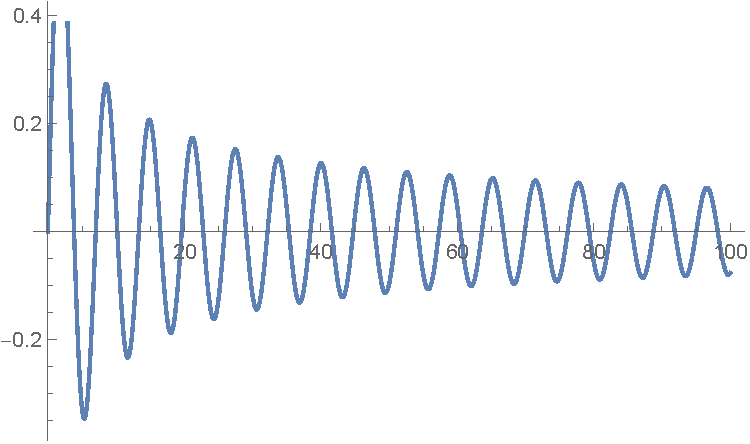
\includegraphics[width=7cm]{Bessel1.pdf}
        \end{center}
        \caption{\label{cylindom}A dartboard like pattern on an annular domain.}
      \end{figure}
      Consider a disk used to model a solid growing bacterial stalk given by a vector $\v{c}(r,\theta)$,
      \begin{equation}
        \v{c}(r,\theta) =r\cos(\theta)\uv{x}  +r\sin(\theta)\uv{y}.
      \end{equation}
      for $r\in[0,R_0]$ and $\theta \in[0,2\pi)$, where $(\uv{x}, \uv{y})$ are Cartesian basis vectors. In this domain the Laplacian of a function $\psi$ takes the following form
      \begin{equation}
        \nabla^2\psi = \pdd{\psi}{r} + \frac{1}{r}\pd{\psi}{r}  + \frac{1}{r^2}\pdd{\psi}{\theta}.
      \end{equation}
      Consider the following generic reaction diffusion type system
      \begin{align*}
        \label{}
        \pd{u}{t} &= \nabla^2 u +F(u,v),\\
        \pd{v}{t} &=D\nabla^2 v +G(u,v),
      \end{align*}
      on this domain. There are no-flux boundary conditions on the domain boundary, $D$ is a positive constant.
      \begin{enumerate}[label=(\alph*)]
        \item{State explicitly the boundary conditions for this problem.
          }
        \item{Consider solutions $u(r,\theta,t) = u_0 +\epsilon u_1(r,\theta,t)$ and $v(r,\theta,t) = v_0 + \epsilon v_1(r,\theta,t)$, where $u_0,v_0$ are homogeneous equilibria of the system. Find the $\order(\epsilon)$ equations and assume their solutions take the form $u_1 =\psi_u(r,\theta)\e^{\lambda t}$ and $v_1 =\psi_v(r,\theta)\e^{\lambda t}$, where $\psi_u$ and $\psi_v$ satisfy
            \begin{equation}
              \nabla^2 \psi_u + k^2\psi_u = 0 \quad \text{and} \quad \nabla^2 \psi_v + k^2\psi_v = 0.
            \end{equation}
            Show that solutions to these eigen-equations take the form
            \begin{equation}
              \psi_{u/v}(r,\theta) = \sum_{n=0}^{\infty}\left[f_{n1}(r)\cos(n\theta) + f_{n2}(r)\sin(n\theta)\right],
            \end{equation}
            where $f_{n\alpha},\alpha= 1,2$ solve the equation
            \begin{equation}
              \label{zfunc}
              \fdd{f_{n\alpha}}{r} + \frac{1}{r}\fd{f_{n\alpha}}{r} + \left(k^2-\frac{n^2}{r^2}\right)f_{n\alpha}=0.
            \end{equation}
          }
        \item{You are told that the observed patterns form a set of concentric rings, as shown in \cref{cylindom}(a). State the form of the permissible spatial patterns $\psi_u$, given that the solution to \cref{zfunc} takes the form
            \begin{equation}
              f_{n\alpha}(z) = A_{n\alpha} J_{n}(k r) + B_{n\alpha} Y_{n}(k r),
            \end{equation}
            with $J_{n}(x)$ and $Y_{n}(x)$ the Bessel functions of the first and second kind. The $0^\text{th}$ Bessel function of the first kind takes the form
            \begin{align}
              J_0(r) = \sum_{m=0}^{\infty}\frac{(-1)^m}{m!\,\Gamma(m+1)}\left(\frac{r}{2}\right)^{2m},\quad  \Gamma(n) = (n-1)!,
            \end{align}
            and the second kind,
            \begin{equation}
              Y_0(r)=\frac{2}{\pi}\left\{[\ln(r/2)+\gamma]J_0(r)+\sum_{k=1}^{\infty}(-1)^{k+1}H_k\frac{(r^2/4)^k}{(k!)^2}\right\},
            \end{equation}
            where $\gamma$ and $H_k$ are constants. Show that the equation for $k$ simplifies to
            \begin{equation}
              \label{bcon}
              J_{1}(k R_0) = 0.
            \end{equation}
          }
        \item{
            A plot of $J_1(r)$ is shown in \cref{cylindom}(b), there is a countable infinity of $k$ values which can solve the boundary condition, \cref{bcon}. Assume there are two stalks whose cross-sectional radii are $R_0=1$ and $R_0=100$. Assume the reaction--diffusion system is such that the Turing conditions satisfied in both cases and are independent of $R_0$. Which domain has more potential patterns?
          }
      \end{enumerate}
    }
    {
      \begin{enumerate}[label=(\alph*)]
        \item{
            The $\theta$ boundary conditions are necessarily periodic,
            \begin{equation}
              u(r,0,t) = u(r,2\pi,t), \mbox{and } v(r,0,t)= v(r,2\pi,t).
            \end{equation}
            The $r$ boundary condition is
            \begin{equation}
              \pd{u}{r}(R_o,\theta,t) =0,
            \end{equation}
            and similar for $v$.
          }
        \item{This is just bookwork from your notes. In an exam you could assume the Fourier series solution just by citing the periodicity of the domain in the $\theta$ coordinates.

          }
        \item{
            I will leave the argument to you as to why, but you should be choosing the $n=0$ modes only so the sin parts are automatically zero. We note that the function $Y_0$ will blow up as $r\rightarrow 0$ so the constant $B_{01}$ must be zero (why don't I care about $B_{02}$\dots?). Thus we have
            \begin{equation}
              \psi_u(r,\theta) = A_{01} J_0(kr).
            \end{equation}
            Now, to get an equation for $k$ we must apply the radial boundary condition (we have of course already enforced the $\theta$ boundary conditions). From the form of $J_0$ we see $\fd{J_0(kr)}{r} = -kJ_1(kr)$. So applying $\fd{u}{r}=0$ at $r=R_o$ yields the required equation.
          }
        \item{

            This relies on your underlying understanding of the Turing mechanism. Remember that satisfying the Turing conditions implies there is some finite domain $k\in[k_{\min},k_{\max}]$ for which patterns will grow in time ($\lambda>0$). Increasing $R_0$ means more zeros of $J_1$ in the same $k$ domain $k\in[k_{\min},k_{\max}]$, thus more likely patterns which are assumed to form due to random changes about the homogeneous equilibrium.  So the $R_0=100$ case should have more patterns all else being equal.
          }
      \end{enumerate}

    }
    %

    %===========================================================================

    %
    \question{Chemotaxis (Exam section B type)}
    {
      Consider the following one-dimensional chemotactic slime mould model,
      \begin{subequations}
        \begin{align}
          \pd{n}{t} &= D\pdd{n}{x} -\alpha\pd{}{x}\left[n\pd{c}{x}\right],\\
          \pd{c}{t} &= \pdd{c}{x} + \gamma c\frac{n^2}{\mu +n^2},
        \end{align}
      \end{subequations}
      where $\alpha,\mu$ are positive constants and $\gamma \in \mathbb{R}$.
      \begin{enumerate}[label=(\alph*)]
        \item{Let $n=n_0$ be a spatially homogeneous equilibrium state for $n$. Suppose $n$ is in this equilibrium state. If we further assume that $c$ has a spatially homogeneous profile, which initially takes a value $c_0$, then show that
            \begin{equation}
              c= c_0\e^{rt},\mbox{ where } r = \gamma\frac{n_0^2}{\mu+n_0^2}.
            \end{equation}
          }
        \item{Consider solutions of the form
            \begin{equation}
              n(x,t) = n_0 + \epsilon f(t)\sum_{k}\e^{\i kx},\quad c(x,t) = c_0\e^{rt} + \epsilon g(t)\sum_{k}\e^{\i kx},
            \end{equation}
            where $\epsilon\ll1$.
            Show that, for each $k$, the $\order(\epsilon)$ equations are:
            \begin{subequations}
              \label{modeqs}
              \begin{align}
                \pd{f}{t} &= -Dk^2 f +\alpha n_0 k^2 g,\\
                \pd{g}{t} &= -\left(k^2 -r\right)g  + \frac{2n_0 c_0}{\mu + n_0^2}\left(\gamma -r\right)\e^{rt}f.
              \end{align}
            \end{subequations}
          }
        \item{Show that the system, \cref{modeqs}, can be reduced to a single ordinary differential equation for $f$ in the form
            \begin{align}
              \label{modeq}
              \fdd{f}{t} + a(k)\fd{f}{t} + \left[b(k)\e^{rt} + c(k)\right]f=0,
            \end{align}
            where
            \begin{align}
              &a(k) = \left[Dk^2 + \left(k^2 - r\right)\right],\quad b(k) =\alpha n_0 \beta\left(r-\gamma\right)k^2, \quad \beta = \frac{2n_0 c_0}{\mu + n_0^2},\\
              &c(k) =   \left(k^2 -r\right)D k^2.
            \end{align}
          }
        \item{One technique for assessing the behaviour of each mode could be to make the assumption that the coefficients of the equation
            \begin{equation}
              \fdd{f}{t} + a(k)\fd{f}{t} + \left[b(k)\e^{rt} + c(k)\right]f=0
            \end{equation}
            vary at a rate slower than the function $f$ and its derivatives. Why is this assumption incorrect in this case?
          }
        \item{We now assume $r/\gamma=1$ and consider the problem on a domain of length $L$ with no-flux boundary conditions. State a condition for which all growth modes will be stable.
          }

      \end{enumerate}
    }
    {
      \begin{enumerate}[label=(\alph*)]
        \item{If $c$ is not spatially varying then $\pd{c}{x}=0$ so $n$ can be any constant. The equation for $c$ then reduces to
            \begin{equation}
              \fd{c}{t} = \gamma c \frac{n_0^2}{\mu+n_0^2},
            \end{equation}
            whose solution is
            \begin{equation}
              c= A\e^{rt},\quad r = \gamma\frac{n_0^2}{\mu+n_0^2}.
            \end{equation}
            The initial condition $c_0$ sets $A$ and gives the required answer.
          }
        \item{
            To linear order,
            \begin{align}
              \pd{n}{t} &= \epsilon\pd{f}{t}\sum_{k}\e^{\i kx}, & \pd{c}{t} &= rc_0\e^{rt}+ \epsilon\pd{g}{t}\sum_{k}\e^{\i kx},\nonumber\\
              \nabla^2 n &= -\epsilon k^2 f(t)\sum_{k}\e^{\i kx},& \nabla^2 c &= -\epsilon k^2 g(t)\sum_{k}\e^{\i kx},\nonumber\\
              \pd{c}{x} &= -\epsilon\i k g(t)\sum_{k}\e^{\i kx}, & n\pd{c}{x} &\approx \epsilon n_0\i k g(t)\sum_{k}\e^{\i kx} + \order(\epsilon^2),\nonumber\\
              &&\pd{}{x}\left[n\pd{c}{x}\right] &\approx -\epsilon n_0 k^2 g(t)\sum_{k}\e^{\i kx} + \order(\epsilon^2).
            \end{align}
            The last term needed is a little tricky. If we just denote temporarily $n_0$ and $c_0^*$ as the zeroth order terms and $n_1$, $c_1$ the corrections
            \begin{equation}
              c\frac{n^2}{\mu + n^2} \approx c_0^*\frac{n_0^2}{\mu + n_0^2} + \epsilon\left[n_1c_0^*\left(\frac{2n_0}{\mu + n_0^2} - \frac{2n_0^3}{(\mu+n_0^2)^2}\right) + c_1\frac{n_0^2}{\mu+n_0^2},
              \right].
            \end{equation}
            then using our definition of $r$ the $\order(\epsilon)$ correction is
            \begin{equation}
              \frac{2n_1n_0 c_0^*}{\mu + n_0^2}\left(1 - \frac{r}{\gamma}\right) + c_1\frac{r}{\gamma}
            \end{equation}
            and substituting back in $c_0^*,n_1,c_1$ the order $\epsilon$ term is
            \begin{equation}
              \frac{2n_0 c_0}{\mu + n_0^2}\left(1 - \frac{r}{\gamma}\right)\e^{rt}f(t)\sum_{k}\e^{\i kx} + \frac{r}{\gamma}g(t)\sum_{k}\e^{\i kx}.
            \end{equation}
            Collecting all $\order(\epsilon)$ terms we find for each $k$ that
            \begin{align}
              \pd{f}{t} &= -Dk^2 f +\alpha n_0 k^2 g,\\
              \pd{g}{t} &= -\left(k^2 -r\right)g  + \frac{2n_0 c_0}{\mu + n_0^2}\left(\gamma -r\right)\e^{rt}f.
            \end{align}
          }
        \item{
            Taking the derivatives of the first equation we get
            \begin{equation}
              \pdd{f}{t} = -Dk^2 \pd{f}{t} +\alpha n_0 k^2 \pd{g}{t}.
            \end{equation}
            We then substitute in the second equation to find
            \begin{align}
              \pdd{f}{t} = -Dk^2 \pd{f}{t} +\alpha n_0 k^2\left\{-\left(k^2 -r\right)g  + \beta\left(\gamma - r\right)\e^{rt}f\right\},\\
              \implies \pdd{f}{t} = -Dk^2 \pd{f}{t}+\alpha n_0 \beta\left(\gamma - r\right)\e^{rt}k^2f - \alpha n_0 k^2\left(k^2 -r\right)g,
            \end{align}
            where $\beta = \frac{2n_0 c_0}{\mu + n_0^2}$.
            We now use the first equation again to obtain an expression for $g$,
            \begin{equation}
              \alpha n_0 k^2 g =   \pd{f}{t} + Dk^2 f,
            \end{equation}
            so that
            \begin{align}
              \pdd{f}{t} = -\left[Dk^2 + \left(k^2 -r\right)\right]\pd{f}{t}+\left[\alpha n_0 \beta\left(\gamma - r\right)\e^{rt} - \left(k^2 -r\right)D\right]k^2f.
            \end{align}
          }
        \item{
            The coefficient of the $f(t)$ part of the equation contains an exponential term. Since we would expect the constant coefficient case to show exponential growth or decay the assumption of differing rates of change is not valid.
          }
        \item{
            In this case $b(k)=0$. We have an equation with constant coefficients. We seek a solution in the form $\e^{\lambda t}$ for which
            \begin{equation}
              \lambda^2 + a\lambda + c =0,
            \end{equation}
            so
            \begin{equation}
              \lambda = \frac{1}{2}\left[-a \pm \sqrt{a^2 -4c}\right].
            \end{equation}
            If
            \begin{equation}
              k^2-r>0,
            \end{equation}
            then $c$ and $a$ will be positive, and both eigenvalues will have a negative real part.
            The no flux boundary conditions imply $k ={n\pi}/{L}$ so we need the lowest mode $n=1$ to be stable, hence
            \begin{equation}
              \frac{\pi^2}{L^2} -r>0.
            \end{equation}
          }

      \end{enumerate}

    }
    %

    %===========================================================================

    %
    \question{Dynamic Turing analysis}
    {
      Consider the following model for the interaction of a bacterial species $u(x,t)$ and a chemical density $v(x,t)$:
      \begin{subequations}
        \label{chemomodel}
        \begin{align}
          \pd{u}{t} &= \pdd{u}{x} - \pd{}{x}\left[\chi(u,v)\pd{v}{x}\right] + u(1-u),\\
          \pd{v}{t} &=D\pdd{v}{x} + uv\left(\frac{1}{t} -1\right),
        \end{align}
      \end{subequations}
      for $t\in(0,\infty]$, $x\in[0,L]$ and both subject to no-flux boundary conditions. Here $D$ is a constant and $\chi(u,v)$ a smooth  scalar function.
      \begin{enumerate}[label=(\alph*)]
        \item{Describe the physical interpretation of the various terms on the RHS of \cref{chemomodel}.
          }
        \item{\label{homog}
            Assume $u$ is in a stable homogeneous equilibrium. Assume further that $v$ remains homogeneous. Solve for the temporal growth of $v(t)$. You may assume any results derived in your class notes.
          }
        \item{
            We now seek to assess whether temporally transient patterns can form in the system. Assume solutions to \cref{chemomodel}  in the form
            \begin{subequations}
              \label{solassump}
              \begin{align}
                u(x,t) &= 1 + \epsilon u_1(x,t) = 1+  \epsilon\sum_{n=0}^{\infty}f_n(t)\e^{\i k_nx},\\
                v(x,t) &= v_0(t) + \epsilon v_1(x,t)= v_0(t)+  \epsilon\sum_{n=0}^{\infty}g_n(t)\e^{\i k_n x},
              \end{align}
            \end{subequations}
            where, $k_n=n\pi/L$,  $\epsilon\ll1$, and $v_0(t)$ is the homogeneous growth function found in part \ref{homog}. Show the order $\epsilon$ equations take the form:
            \begin{align*}
              \fd{f_n}{t} &= -k_n^2 f_n + k_n^2\chi(u_0,v_0)g_n  - f_n,\\
              \fd{g_n}{t} &= -Dk_n^2 g_n +\left(g_n +f_n v_0(t)\right)\left(\frac{1}{t}-1\right).
            \end{align*}
          }
        \item{
            Assume $\chi(u,v)=1$. Demonstrate that the system \emph{can} exhibit  transient patten formation under the assumption of solutions in the form of \cref{solassump}.

            \emph{Hint}: You do not need to solve for $f_n$ and $g_n$ for general $t$, just consider their approximate behaviour at small $t$ and large $t$. You may assume the solutions to $g_n$ and $f_n$ remain $>0$ for all $t$.

          }
      \end{enumerate}
    }
    {
      No solution provided.
    }

\end{enumerate}
\end{document}
